\chapter{ABC}

This chapter will outline a series of illustrative ABC experiments. These examples demonstrate the core concepts from introduced in section \ref{ApproximateBayesianComputation}, demonstrate ABC can sample from complex distributions and build a boutique code base which is the foundations of this project. The code for the figures in this section can be found at \url{https://github.com/tomconnell/abc-toy-problems}.

%This chapter will outline a series of illustrative ABC experiments. These demonstrate the core concepts touched on in the introduction, demonstrate ABC can sample from complex distributions and build a boutique code base which is the foundations of this project.

%In this section I describe experiments in adequate detail for others to undertake, the necessary details to meet preproducility \citep{Stark2018}.

%For transparency and absolute reproducibility I heed the advice of \citet{Buckheit1995}:
%\begin{displayquote}
%\textit{An article about computational science in a scientific publication is not the scholarship itself, it is merely advertising the scholarship. The actual scholarship is the complete development environment and the complete set of instructions which generated the figures.}
%\end{displayquote}
%The MATLAB code for all figures in this section can be found at \url{https://github.com/tomconnell/dram}.

\section{Toy problem 1: 1D Gaussian}
As a first example consider we have observed $n = 100$ realizations from the Gaussian distribution, making our model: $\bm{g_s} = p(\bm{y^*}|\bm{\theta}) \sim \mathcal{N}(\mu,\sigma)$, with unknown model parameters $\bm{\theta} = [\mu,\sigma]$. Given that it is easy to simulate this model, it is possible to leverage ABC algorithms to estimate the unknown model parameters. A synthetic dataset for this problem is created with $\mu = 5$ and $\sigma = 2$. The summary statistics sample mean, $\bar{\mu}$, and sample standard deviation, $\bar{\sigma}$, are used, $\bm{S}(\bm{y}) = [\bar{\mu},\bar{\sigma}]$. These are sufficient statistics for the unknown model parameters. Figure \ref{toy1-fig1} plots the ABC posterior obtained from using algorithm \ref{ABCrejectionsampler}, the traditional form of an ABC rejection sampler, compared to the analytical likelihood. The distance between simulated summary statistics and observed summary statistics is evaluated marginally for simplicity. Throughout this thesis I do not consider the joint distribution and correlation structure present in the distance between summaries. Our distance measure for this example takes the form $\text{d}(\bm{S}(\bm{y}),\bm{S}(\bm{y^*})) = |S_1(\bm{y^*}) - S_1(\bm{y})| +| S_2(\bm{y^*}) - S_2(\bm{y})|$. A uniform prior is used to give equal probability to a bounded area, $p(\mu) = \mathcal{U}(0,10)$ and $p(\sigma) = \mathcal{U}(0,10)$. Figure \ref{toy1-fig2} explores the impact of varying the tolerance for this problem.\par

Figure \ref{toy1-fig1} demonstrates that with sufficient statistics and a low tolerance ABC can accurately resolve the posterior using only the ability to simulate data. However, as figure \ref{toy1-fig2} demonstrates, high tolerances erode posterior accuracy and uncertainty is over-estimated. However, it is true that increasing the tolerance increases the acceptance rate and hence relaxes computational resources. In this case the acceptance rate with $\epsilon = 0.1$ was $0.02\%$, while the acceptance rate with $\epsilon = 1$ was $2.02\%$. Under a model which is expensive to simulate from, walking the tightrope between accuracy and efficiency becomes important and needs to be carefully examined. In spite of shortcomings, the strengths of the ABC rejection sampler has led to significant scientific results in genetics \citep{Fu1997,Weiss1998a,Pritchard1999a}.

\begin{figure}[H]
	\centering
	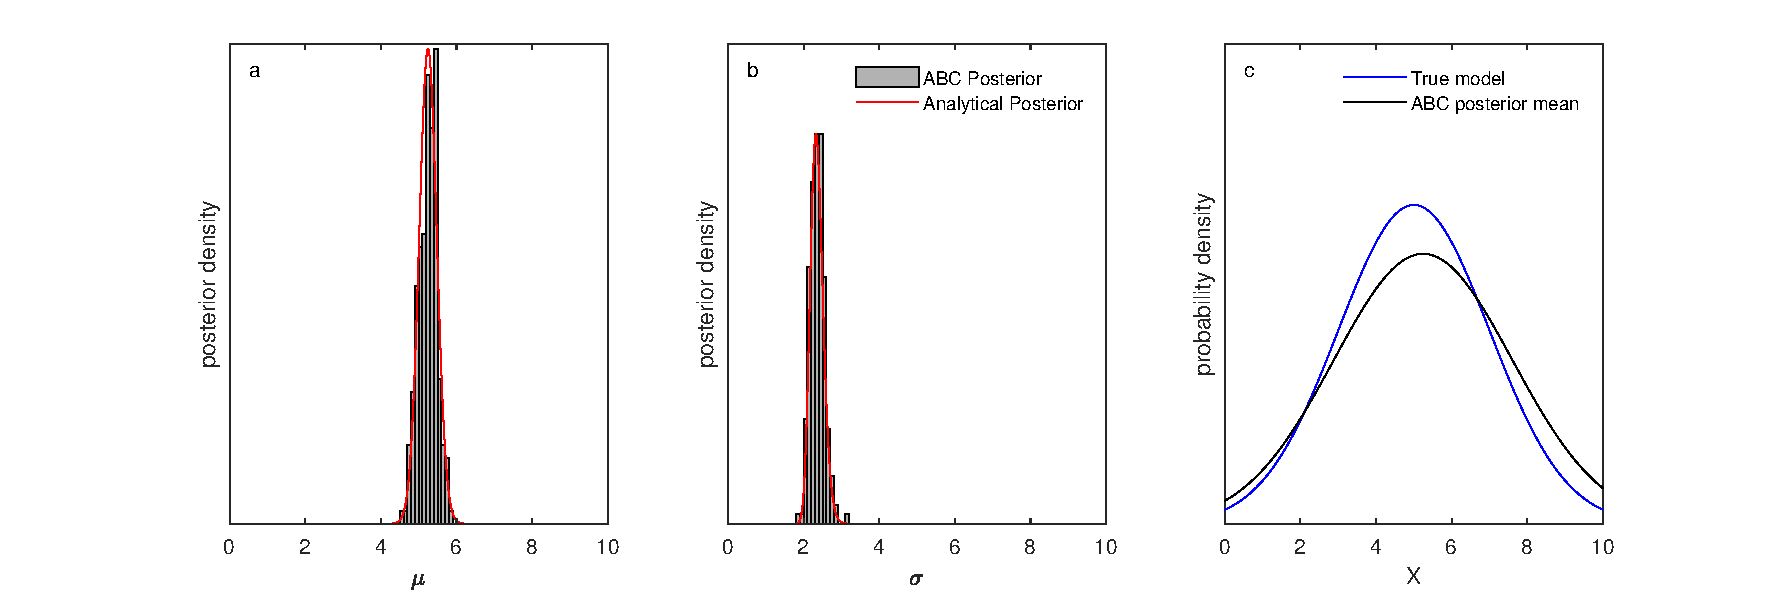
\includegraphics[scale=0.6]{rejectionsampler.pdf}
	\caption{Posterior comparison between ABC and traditional likelihood inference for estimating the parameters, $\bm{\theta} = [\mu,\sigma]$, for a Gaussian model given $n = 100$ observations, $\bm{y}$. The ABC algorithm, algorithm \ref{ABCrejectionsampler}, uses 1 million repetitions and a tolerance $\epsilon = 0.1$. The likelihood takes the form $\mathcal{L}(\bm{\theta}|\bm{Y}) = (2\pi\sigma^2)^{-n/2}\ \text{exp}\big[-\frac{1}{2\sigma^2}\sum_{i = 1}^{n}(y_i-\mu)^2\big]$. (a) Marginal posterior compared to marginal ABC posterior for unknown parameter $\mu$. (b) same as (a) but for unknown parameter $\sigma$. (c) Mean of the joint ABC posterior compared to true model, $\mathcal{N}(5,2)$.}
	\label{toy1-fig1}
\end{figure}

\begin{figure}[H]
	\centering
	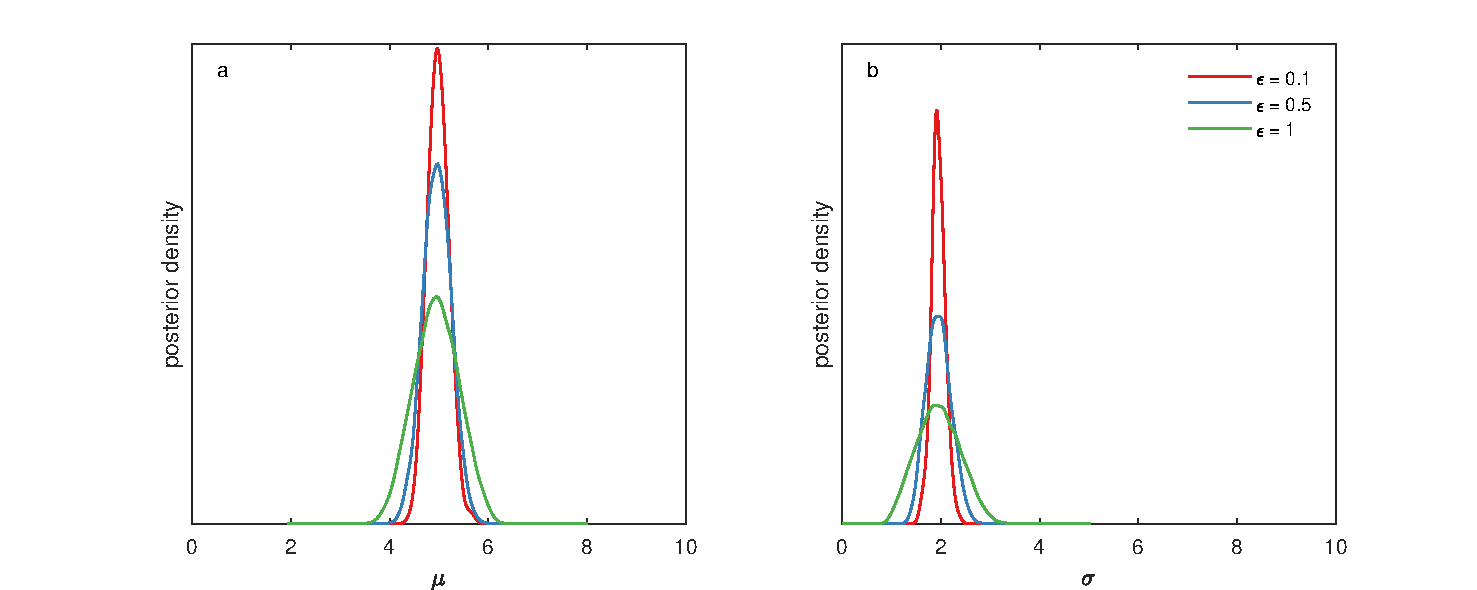
\includegraphics[scale=0.7]{tolerancecomparison.pdf}
	\caption{The effect of varying the tolerance $\epsilon$ when estimating $\bm{\theta} = [\mu,\sigma]$ to a Gaussian model given given $n = 100$ observations, $\bm{y}$. Three tolerances are considered, $\epsilon = 0.1$, $\epsilon = 0.5$, $\epsilon = 1$. (a) Kernel density estimate of the marginal ABC posterior for unknown parameter $\mu$. The true value is $\mu = 5$ (b) same as (a) but for unknown parameter $\sigma$. The true value is $\sigma = 2$}.
	\label{toy1-fig2}
\end{figure}

\section{Toy problem 2: Linear regression}
\label{sec-lin-reg}

As a second example consider we have observed some data, $\bm{y}$, from the linear model $\bm{g}(\bm{\theta}) = m\bm{x} + b$ and there is some stochasticity in the measurement process such that $\bm{g_s}(\bm{\theta}) = \bm{g}(\bm{\theta}) + \mathcal{N}(0,\sigma^2)$. Our unknown parameters are $\bm{\theta} = [m,b]$, while $\sigma$ is known. In this case MCMC, which uses local transitions, will be needed to improve acceptance rates \citep{Gilks1995}. MCMC will also be needed when the search spaces are high dimensional, with many unknown parameters, or the posterior is a long way from the prior. For this case we can call upon ABC-MCMC in the form of algorithm \ref{ABC-MCMC} \citep{Marjoram2003,Sisson2010a}. \par

Algorithm \ref{ABC-MCMC} samples the ABC posterior, equation \ref{summary-stat-abc-posterior}. The algorithm relies on evaluating the MH acceptance probability, equation \ref{M-H-acce}. The current examples use Gaussian proposal distributions, $q(\cdot,\cdot)$. As such the proposal distributions cancel out in equation \ref{M-H-acce}. That leaves the prior and the weighting kernel to be evaluated at each time step in the Markov chain. The weighting kernel takes the form of equation \ref{generic-weighting-kernel}. In this case a uniform weighting kernel, $K_U$, is implemented. The interpretation of $K_U$ is the same as the accept/reject step in the rejection sampler: 
\begin{equation}
	K_U = 
	\begin{cases}
		1 & \text{if}\ 	\frac{\text{d}(S_i(\bm{y^*}),S_i(\bm{y}))}				{\epsilon_i} \leq 1\\
		0 & \text{if}\ \frac{\text{d}(S_i(\bm{y^*}) - S_i(\bm{y}))}				{\epsilon_i} > 1
	\end{cases}
\end{equation}
$K_U$ hence forms an indicator function 1 which is equal to $1$ when the distance between statistics, which are fit marginally, is less than the tolerance. Given, $\bm{S} = \{S_1,\dots,S_O\}$, the weighting kernel takes the form:
\begin{equation}
	p(\bm{S}(\bm{y})|\bm{S}(\bm{y^*}),\bm{\theta}) = \prod_{i = 1}^{O} K_U\Big(\frac{\text{d}(S_i(\bm{y}),S_i(\bm{y^*})}{\epsilon_i}\Big)
	\label{weight-kernel}
\end{equation}
As with the 1D Gaussian example it would be possible to use summaries which have a one-to-one correspondence to the unknown parameters. For a given simulation, a linear model could be fit to the simulated data, i.e. the slope and intercept of the fit model could then be used as summaries. However, to demonstrate that this is not necessary, the sample mean, $\bar{\mu}$, and sample standard deviation, $\bar{\sigma}$, are used as summary statistics \citep{vrugt2013toward}. The slope is restricted to a positive value to make these statistics sufficient. \par

Figure \ref{linear-regression} shows ABC-MCMC applied to the linear regression problem. \par

The next section continues to introduce algorithmic consideration into ABC, building toward a geophysically relevant parameter estimation method.\par

%\begin{figure}[H]
%	\centering
%	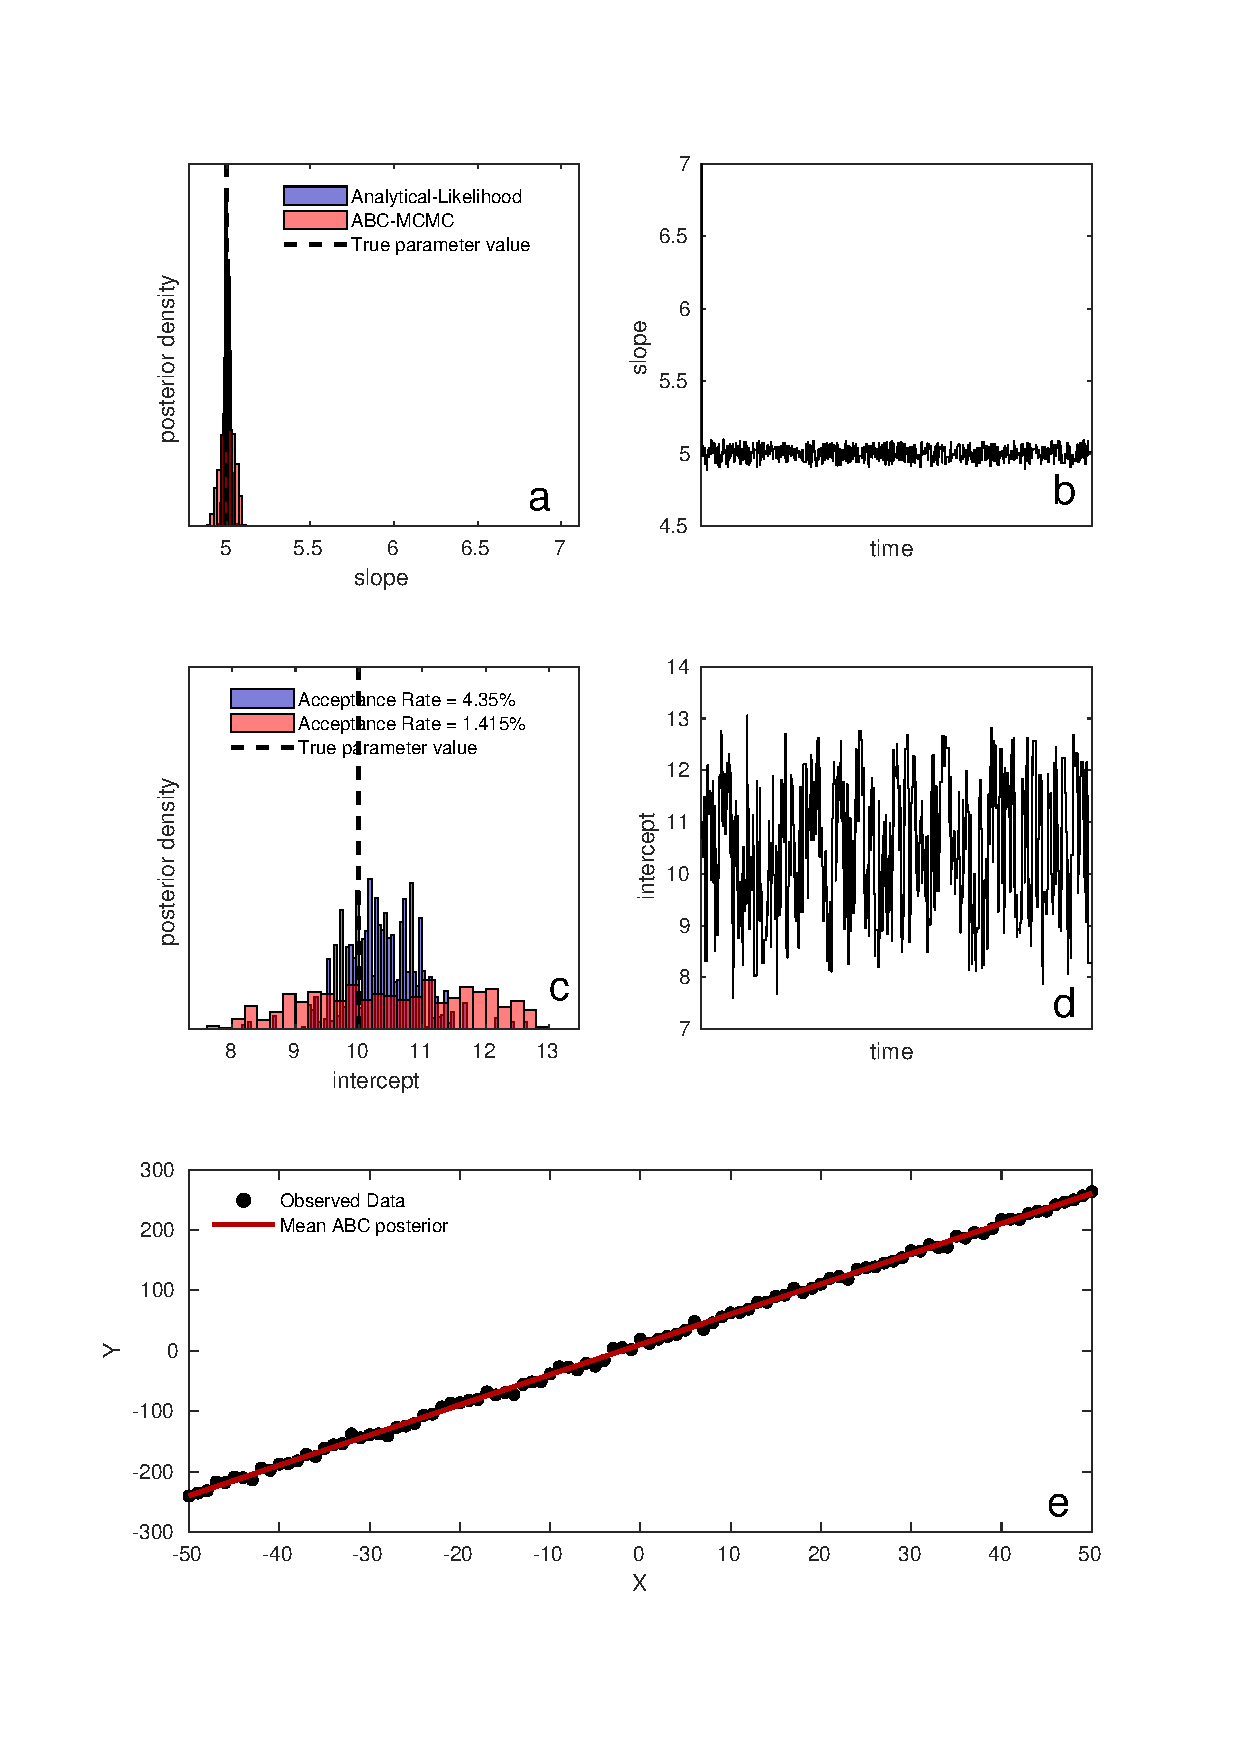
\includegraphics[scale=0.7]{linear-regression.pdf}
%	\caption{Linear regression with ABC. The ABC posterior is also compared to traditional likelihood inference. MCMC is used to sample both posteriors. For ABC the tolerance is $\epsilon = [2\ 2]$. The proposal distribution is $q = \mathcal{N}([0,0],I)$. The Markov chain length is $20\ 000$. (a) The marginal ABC posterior and marginal analytical posterior compared for unknown parameter $m$. (b) Plot of the ABC-MCMC Markov chain through time for $m$. (c) Same as (a) except for unknown parameter $b$. (d) Same as (b) except for unknown parameter $b$. (e) Comparison of the mean ABC posterior model and the observed data generated with $m = 5$, $b = 10$ and $\sigma = 5$.}
%	\label{linear-regression}
%\end{figure}
\begin{figure}[H]	
	\centering
	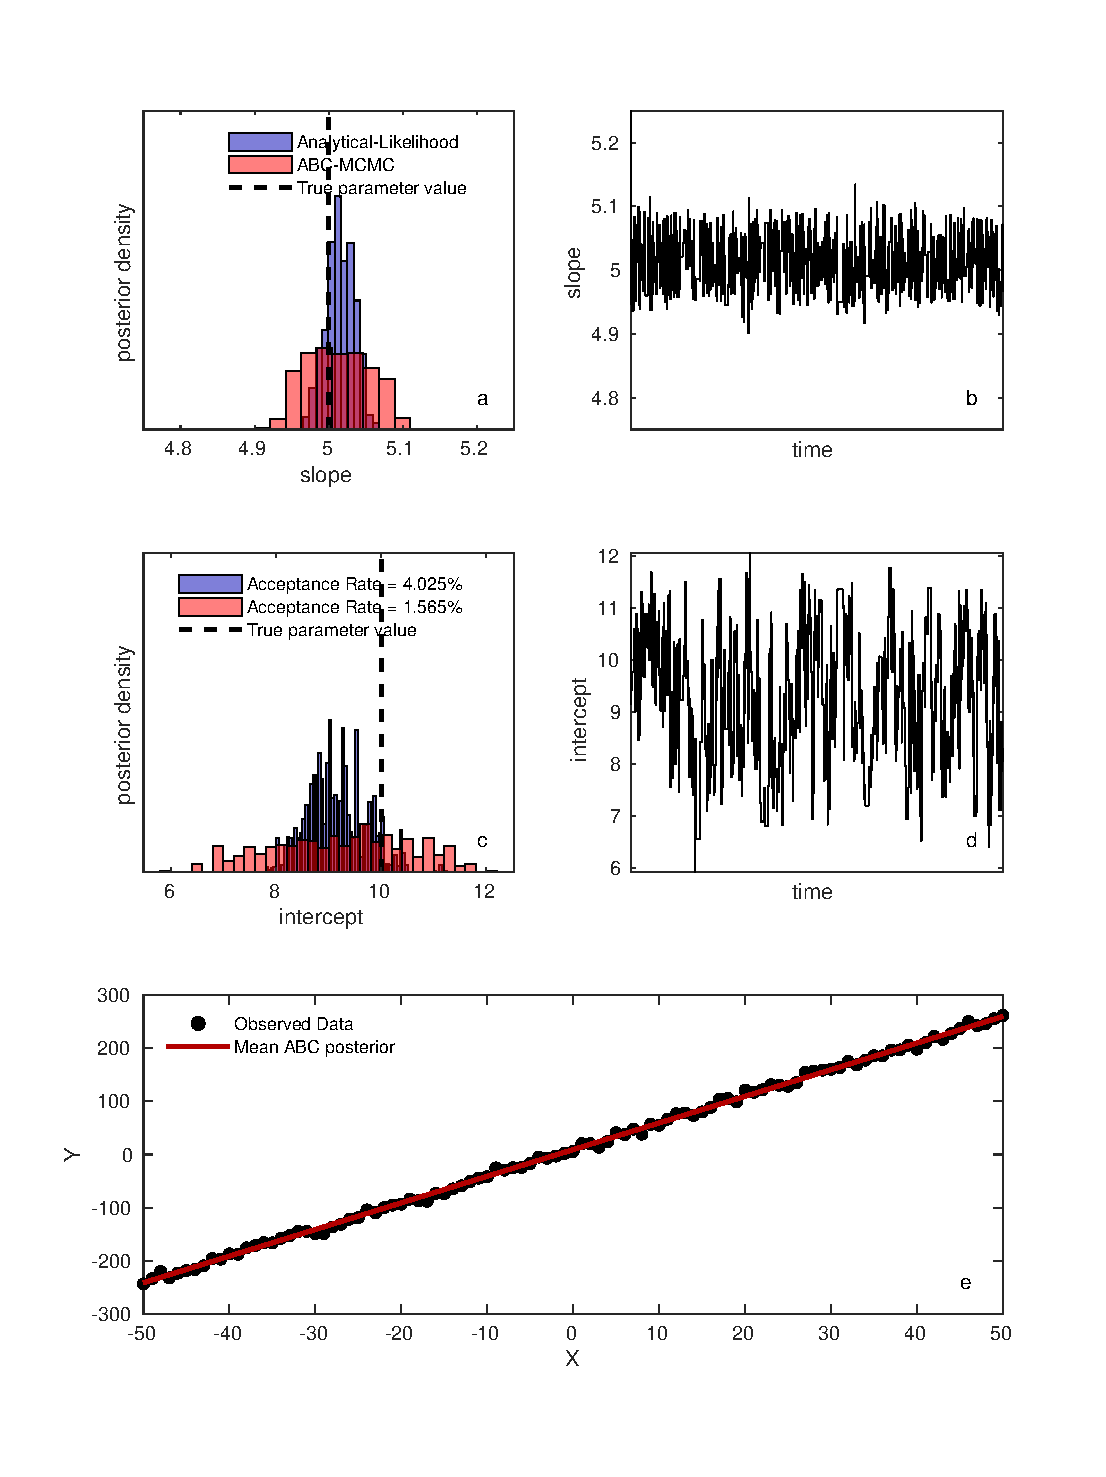
\includegraphics[scale=0.8]{linearregression.pdf}
	\caption{Linear regression with ABC. The ABC posterior is also compared to traditional likelihood inference. MCMC is used to sample both posteriors. For ABC the tolerance is $\epsilon = [2,2]$. The proposal distribution is $q = \mathcal{N}([0,0],I)$. The Markov chain length is $20\ 000$. (a) The marginal ABC posterior and marginal analytical posterior compared for unknown parameter $m$. (b) Plot of the ABC-MCMC Markov chain through time for $m$. (c) Same as (a) except for unknown parameter $b$. (d) Same as (b) except for unknown parameter $b$. (e) Comparison of the mean ABC posterior model and the observed data generated with $m = 5$, $b = 10$ and $\sigma = 5$.}
	\label{linear-regression}
\end{figure}

%This example truly highlights how ABC shifts away from many traditional %Bayesian and frequentist techniques which rely computing data residuals in the %form $\sum (\bm{g}(\bm{\theta})-\bm{y})^2$. This residual is computed in the %analytical linear regression likelihood and is at the heart of all likelihood %functions which are applied in geophysics, equation \ref{likelihood-1} and %equation \ref{likelihood-2}. Instead, ABC opts for informal measures of %'goodness-of-fit' and rely on user-varied tolerances, which guarentee %posteriors close to the true posterior, save for a small degree of bias. The %result of a tolerance $> 0$ and summary statistics which do not always measure %fitness as tightly as a data residual. However the gain is in diagnostic %power. The data residual takes all the information in the data set and mixes %it into a single number, the residual value. However, the form of ABC allows %for the state of the algorithm at any one stage to be evaluated and fitting %statistics marginally means different rules can be set for different %statistics depending on what they mean to the inversion. Understanding how %statistics change through an inversion, the nature in which they diverge, and %the degree to which they spread around the observed value has taught %researches in other disciplines a great deal about the nature of their models %and the systems in which they study. That same central idea should be %transferrable to geophysical parameter estimation problems and may offer room %for more diagnostic inversion schemes, one with a greater deal of user control %and greated deal of interprebable meaning. \\

\section{Toy problem 3: Bivariate Gaussian}
% Introduce the problem
As a third example, consider we have observed $n = 100$ realizations from a bivariate Gaussian distribution $[X,\ Y] = \mathcal{N}(\bm{\mu},\bm{\Sigma})$ with $\bm{\mu} = \begin{bmatrix}
\mu_X,\ \mu_Y
\end{bmatrix}^T$ and $\bm{\Sigma} = \begin{bmatrix}
\sigma^2_X & \rho\sigma_X\sigma_Y\\
\rho\sigma_X\sigma_Y & \sigma^2_Y
\end{bmatrix} $ where both $\bm{\mu}$ and $\bm{\sigma}$ are unknown, $\bm{\theta} = [\bm{\mu},\bm{\Sigma}]$. The causative model has parameters $\bm{\mu} = [2.5,\ 7.5]$, $\sigma_X = 4$, $\sigma_Y = 6$ and $\rho = 0.9$. Figure \ref{init-qualms}(a) plots the causative model and the $n = 100$ realizations which constitute the observed data. This example has 5 unknown parameters in total and ABC-MCMC for efficient sampling. The weighting kernel takes the same form as equation \ref{weight-kernel} and summaries with a one-to-one correspondence to the unknown parameters are used, the marginal sample means, $\bar{\mu_X}$ and $\bar{\mu_Y}$, sample standard deviations, $\bar{\sigma_X}$ and $\bar{\sigma_Y}$, and sample covariance, $\bar{\text{cov}}(X,Y)$. The prior distribution, $p(\bm{\theta}) = \mathcal{U}(0,10)$, is used to provide equal probability to a bounded area for all unknowns beside correlation, $\rho$, which bounded as $p(\rho) = \mathcal{U}(-1,1)$. Figure \ref{init-qualms}(b) shows the results of the first 10 000 time steps from an ABC-MCMC. This figure shows the Markov chain does not make an accepted proposal during the first 4,500 time steps.
%% Figure a of the observed data and figure b of the stuck chain
\begin{figure}[H]
	\centering
	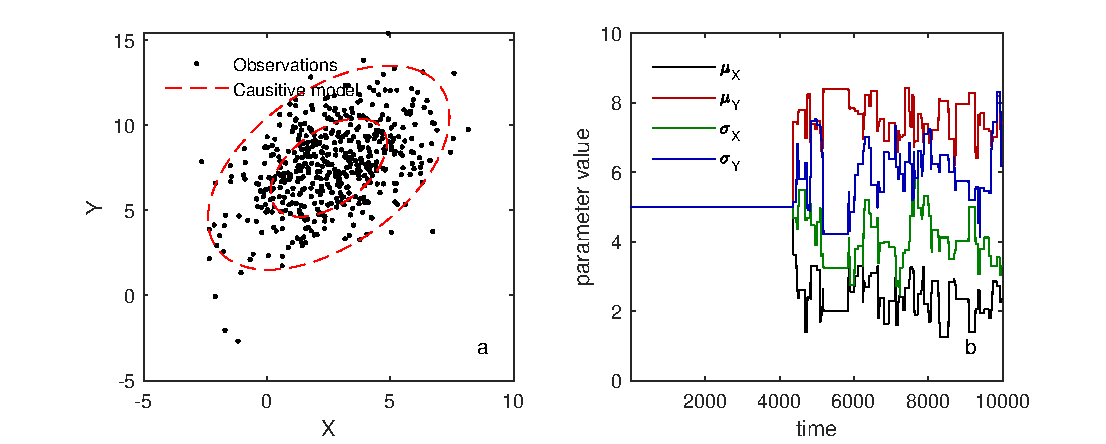
\includegraphics[scale=0.85]{initqualms.pdf}
	\caption{(a) Observed data from the underlying causative model, whose parameters will be the inference target. (b) First 10 000 iterations of an ABC-MCMC scheme with a uniform kernel. The algorithm initially struggles to find a region of non-zero probability from a random starting position within the parameter space.}
	\label{init-qualms}
\end{figure}

%Figure of the chain becoming stuck at the beggining
While ABC-MCMC and the uniform weighting kernel $K_U$ offer improved acceptance rates compared to a rejection scheme, the algorithm can run into an initialization problem, as highlighted in figure \ref{init-qualms}(b). This is a problem which occurs when using a weighting kernel $p(\bm{y}|\bm{y^*},\bm{\theta})$ with compact support. This problem originates when the chains starting position is far from a region where the weighting kernel offers support, within the bounds of \pm\epsilon. The chain then cannot make efficient local transitions via the proposal distribution to the region of high posterior density. \citet{Sisson2010a} offer several strategies to overcome this problem. For example, repeated simulations can be made from the prior until a starting position is found which is within \pm \epsilon. Alternatively, \citet{Bortot2007} augment the posterior to $p_{ABC}(\bm{\theta},\bm{y^*},\epsilon|\bm{y})$, introducing ideas akin to simulated annealing or simulated tempering to ABC via a variable \epsilon. Even if the initialization is overcome, the acceptance rate under $K_U$ with low $\epsilon$ will be low when moving through regions of very diffuse posterior density.
Here, I circumvent the initialization problem which occurs in weighting kernels with compact support by favoring a weighting kernel $p(\bm{y}|\bm{y^*},\bm{\theta})$ with infinite support. That is, the weight diminishes with distance, however it never reaches zero. There are many kernels which have this required property. Here I use a weighting kernel based on the Gaussian distribution, $K_G$. This choice is advantageous as the log-distance can be evaluated for stable computation in sampling algorithms. This mirrors the stable implementation of likelihood values, expanded upon in \hyperref[tf3]{Technical figure 3}. This shift to $K_G$ will allow the algorithm, if in an area of low posterior density, to make efficient local transitions toward an area of high probability density.\par

%While ABC-MCMC and the uniform weighting kernel $K_U$ offers improved acceptance rates compared to a rejection scheme, it is not without faults. Firstly, it can suffer from an initialization problem, as highlighted in figure \ref{init-qualms}(b). Compounding this, the acceptance rate can rapidly decline past a certain threshold as tolerance is decreased. This is a symptom of the same problem as initialization. Each move is either flat out rejected or is determined to be part of the posterior. This makes it prone to becoming stuck when in the tails of the posterior distribution. This is especially problematic in high-dimensional search spaces where the posterior density is an extraordinarily small volume. Ideally, if in a poor spot, the algorithm should be able to make local transitions toward an area of high probability density. However, this adjustment will involve abandoning the $K_U$. A weighting kernel which offers infinite support is needed. That is, the weight diminishes with distance, however it never reaches zero. Fortunately many functions have the required properties. In this text we favour a  weighting kernel based on the Gaussian distribution, $K_G$. This choice is advantageous as the log-distance can be evaluated for stable computation in sampling algorithms. This implementation mirrors the stable implementation of likelihood values, expanded upon in \hyperref[Box2]{Box 2}.\\

For an observed dataset $\bm{S}(\bm{y})$ and simulated dataset $\bm{S}(\bm{y^*})$, where $\bm{S} = \{S_1,\dots,S_O\}$, the Gaussian weighting kernel is computed as:
\begin{equation}
p(\bm{S}(\bm{y})|\bm{S}(\bm{y^*}),\bm{\theta}) = K_G\big(\text{d}(\bm{S}(\bm{y}),\bm{S}(\bm{y^*}))\big) \propto \prod_{i = 1}^{O} \text{exp}\Big[-\frac{1}{2}\Big(\frac{\text{d}(S_i(\bm{y}),S_i(\bm{y^*}))}{\epsilon_i}\Big)^2\Big]
\end{equation}
Figure \ref{KuVSKg-1} compares $K_U$ and $K_G$ over the first 10 000 time steps in an ABC-MCMC algorithm targeting the parameters of a bivariate Gaussian distribution, $\bm{\theta} = \begin{bmatrix}
\bm{\mu}\ \bm{\Sigma}
\end{bmatrix}$. $K_G$ does not suffer from the same initialization problem as $K_U$. $K_G$ also has an improved acceptance rate and better mixing when compared to $K_U$. Figure \ref{KuVSKg-2} demonstrates that with time both kernels converge to the same posterior after 1,000,000 time steps.\par

The posterior sampled in both figure \ref{KuVSKg-1} and \ref{KuVSKg-2} shows an insensitivity to $\rho$. This is a direct result of the insufficiency of the selected summary statistics for that parameter. This reinforces that while a smaller $\epsilon$ improves the approximation of  $p(\bm{\theta}|\text{d}(S(\bm{y}),S(\bm{y^*}))<\epsilon)$ to $ p(\bm{\theta}|S(\bm{y}))$, if the summary statistics are not informative such that $p(\bm{\theta}|S(\bm{y})) \approx p(\bm{\theta}|\bm{y})$, then the parameter inference will be inaccurate. In this case the statistic $\text{cov}(X,Y)$ which should be sensitive to $\rho$, remains overwhelmed by $\sigma_X$ and $\sigma_Y$. Here the sample correlation, $\bar{\rho}$, would have provided a better summary statistic choice. 

\begin{figure}[H]
	\centering
	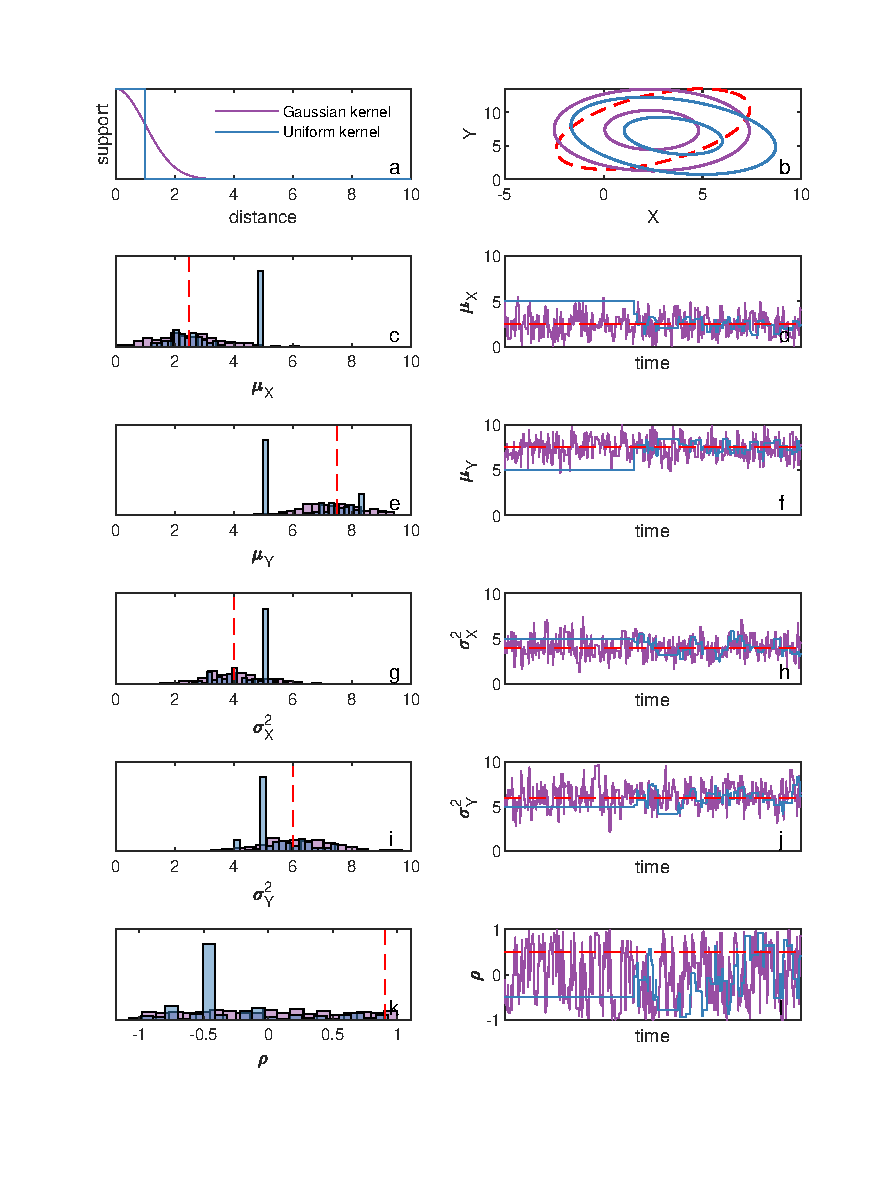
\includegraphics[scale=1]{initalchains.pdf}
	\caption{Comparison between ABC-MCMC with a weighting kernel based on a uniform distribution, $K_U$, with compact support, and a Gaussian distribution, $K_G$, with infinite support. Both Markov chains target the ABC posterior for the parameters to a bivariate Gaussian distribution, $\bm{\theta}$ = [$\bm{\mu}, \bm{\Sigma}$], based on the observed data in figure \ref{init-qualms}(a). The comparison in this figure is limited to the first 10,000 time steps of the respective Markov chains. (a) Plots the support offered by $K_U$ and $K_G$ over distance, d($\bm{y}$,$\bm{y^*}$), for $\epsilon=1$. (b) plots the causative model, red, compared to the mean marginal posterior model for the first 10,000 time steps of the Markov chain based on $K_U$ and $K_G$. (c),(e),(g),(i),(k) plots the marginal posterior sampled by the Markov chain over the first 10,000 time steps for both $K_U$ and $K_G$. (d),(f),(h),(j),(l) plots the Markov chain position through time for the first 10,000 time steps. This figure highlights how ABC based on $K_G$ overcomes the initialization problem, seen in the Markov chain traces for $K_U$, and offers improved acceptance rates and mixing relative to $K_U$.}
	%\caption{Comparison between the Uniform and Gaussian kernel when targeting the parameters to a Gaussian distribution with ABC-MCMC. This is the first 10 000 time steps. This demonstrates how inference based on the Gaussian kernel with infinite support, (a), overcomes the initialization problem the uniform kernel suffers from. The improved mixing and acceptance rate can be seen in the Markov chain traces, (d,f,h,j,l).}
	\label{KuVSKg-1}
\end{figure}

\begin{figure}[H]
	\centering
	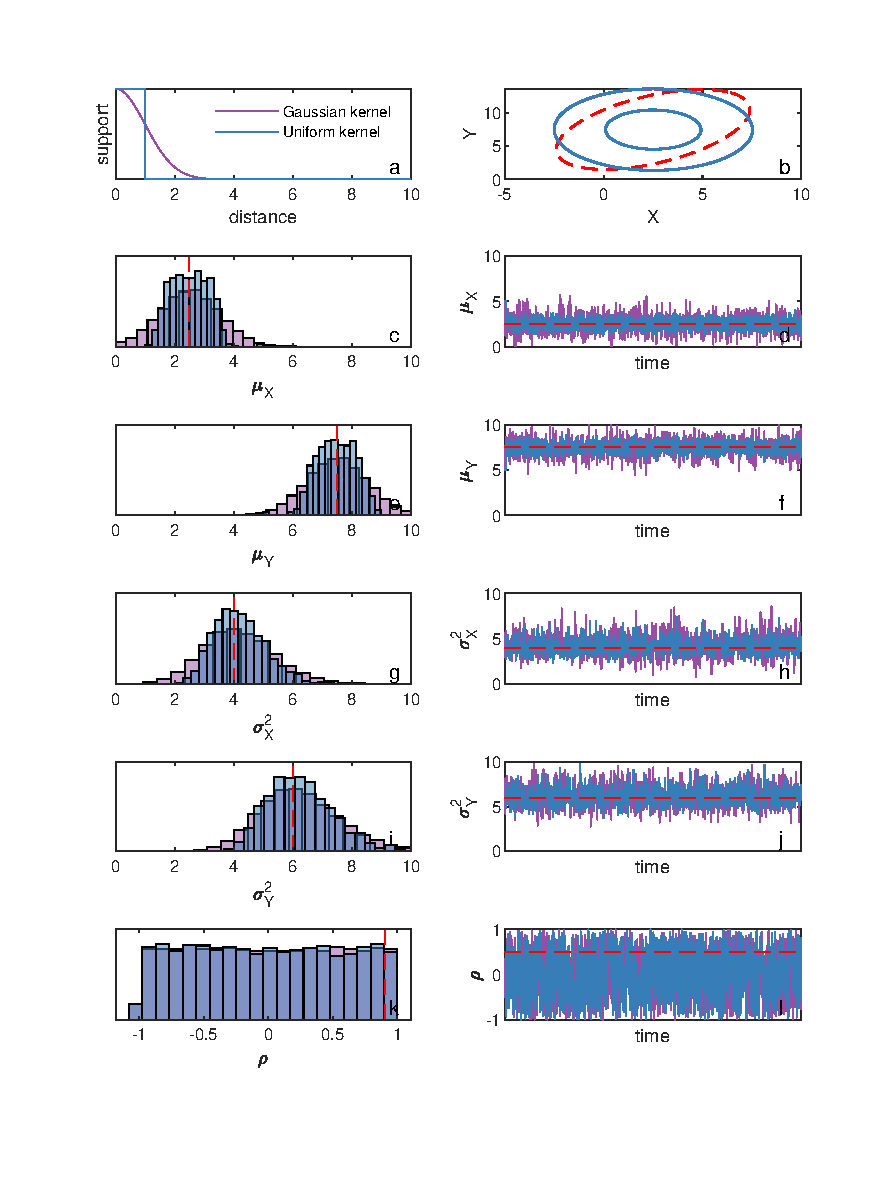
\includegraphics[scale=1]{fullschains.pdf}
	\caption{ This figure is a re-creation of figure \ref{KuVSKg-1} for 1,000,000 time steps. It is a comparison between ABC-MCMC with a weighting kernel based on a uniform distribution, $K_U$, with compact support, and a Gaussian distribution, $K_G$, with infinite support. Both Markov chains target the ABC posterior for the parameters to a bivariate Gaussian distribution, $\bm{\theta}$ = [$\bm{\mu}, \bm{\Sigma}$], based on the observed data in figure \ref{init-qualms}(a). (a) Plots the support offered by $K_U$ and $K_G$ over distance, d($\bm{y}$,$\bm{y^*}$), for $\epsilon=1$. (b) plots the causative model, red, compared to the mean marginal posterior model for the full 1,000,000 time steps of the Markov chain based on $K_U$ and $K_G$. (c),(e),(g),(i),(k) plots the marginal posterior sampled by the Markov chain over the full 1,000,000 time steps for both $K_U$ and $K_G$. (d),(f),(h),(j),(l) plots the Markov chain position through time for the full 1,000,000 time steps. This figure highlights how the two methods converge to the same solution, in contrast to figure \ref{KuVSKg-1}. The difference the marginal posterior of $K_U$ and $K_G$ is a result of the wider support offered by the Gaussian kernel compared to the equivalent uniform kernel (a).}
	%\caption{Comparison between the Uniform and Gaussian kernel for 1 000 000 time steps of an ABC-MCMC algorithm. This demonstrates how the two methods converge to the same solution, in contrast to figure \ref{KuVSKg-1}. The difference in posteriors is a result of the wider support the Gaussian kernel offers compared to the equivalent uniform kernel, (a).}
	\label{KuVSKg-2}
\end{figure} 

\section{Toy problem 4: Banana distribution}
\label{banana-section}

As a fourth example we design a more challenging problem, one for which there are no immediate or obvious summary statistics. Consider we have $n = 1000$ observations from a 'banana' distribution, Figure \ref{banana-data}. This is a standard distribution to test the performance of MCMC as it is moderately non-linear and the posterior can be analytically defined \citep{Haario1999}. To define the banana distribution, we start with a 2-dimensional Gaussian distribution:
\begin{equation}
\begin{bmatrix}
x\ y
\end{bmatrix}=\mathcal{N}(\bm{\mu},\bm{\Sigma}),\ \bm{\mu} = \begin{bmatrix}
\mu_X,\ \mu_Y
\end{bmatrix}^T,\ \bm{\Sigma} = \begin{bmatrix}
\sigma^2_X & \rho\sigma_X\sigma_Y\\
\rho\sigma_X\sigma_Y & \sigma^2_Y
\end{bmatrix} 
\label{gauss-banana}
\end{equation}
The Gaussian co-ordinates $x$ and $y$ are then twisted to produce a more nonlinear target, $X$ and $Y$, using:
\begin{equation}
X = b_1x
\label{x-banana}
\end{equation}
\begin{equation}
Y = y/b_1-b_2(b_1^2x^2+b_1^2)
\label{y-banana}
\end{equation}
In total the parameters which define this model are $\bm{\mu}$, $\bm{\Sigma}$ and the 'bananity' parameters $\begin{bmatrix}
b_1\ b_2
\end{bmatrix}$. Here the unknown target parameters are $\bm{\mu} = \begin{bmatrix}
0\ 0
\end{bmatrix}^T$,
$\bm{\Sigma} = \begin{bmatrix}
\sigma^2_X & \rho\sigma_X\sigma_Y\\
\rho\sigma_X\sigma_Y & \sigma^2_Y
\end{bmatrix}$ while $\begin{bmatrix}
b_1\ b_2
\end{bmatrix}$ = $\begin{bmatrix}
1\ 1
\end{bmatrix}$. 

\begin{figure}[H]
\centering
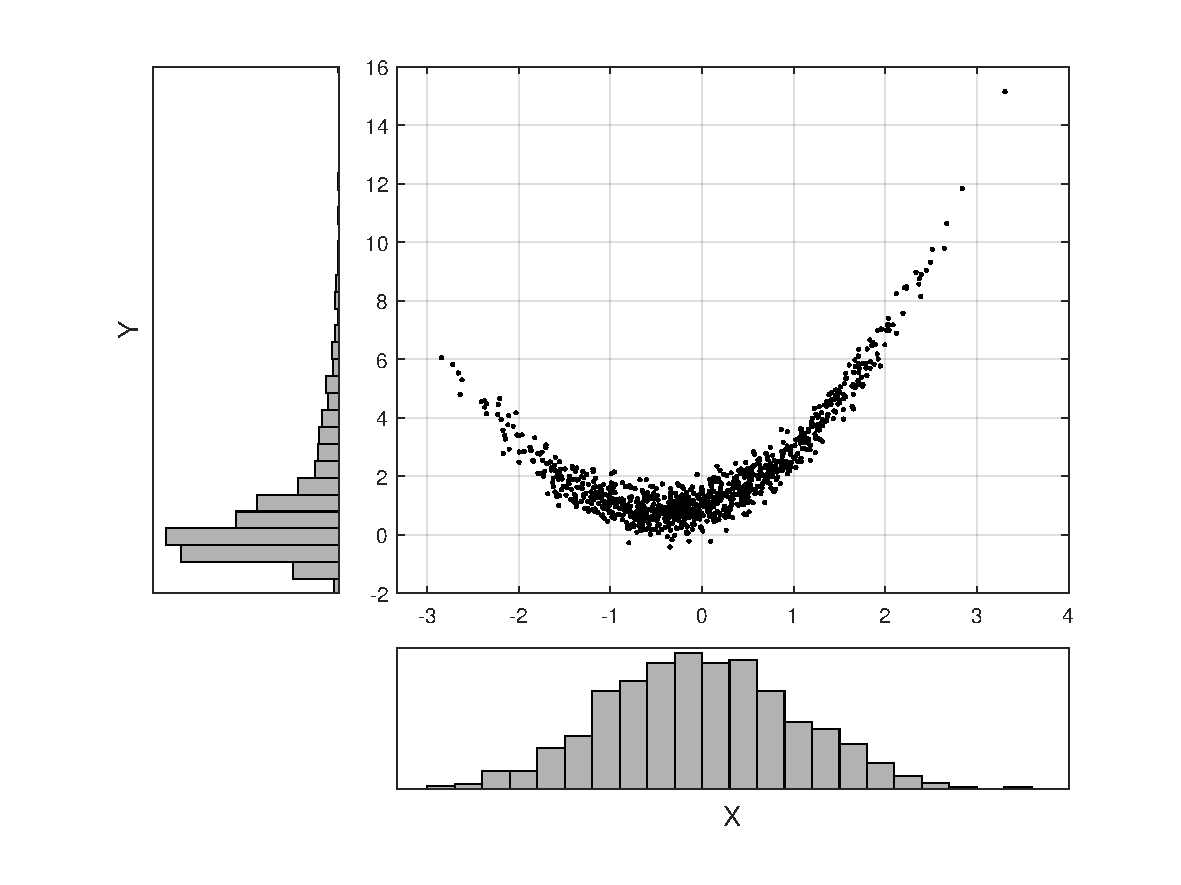
\includegraphics[scale=0.7]{observeddata.pdf}
\caption{$n = 1000$ observations from the 'banana' distribution, analytically defined by equations \ref{gauss-banana}, \ref{x-banana}, \ref{y-banana}. 
This problem is more challenging as there is no immediately apparent sufficient statistics to facilitate ABC estimation of the unknown parameters.}
\label{banana-data}
\end{figure}

To apply ABC inference a set of reasonably sufficient statistics is required. In the previous examples it has been possible to use the sample values for each of the unknown parameters, however, this proved to be insufficient in a trial run. In the ABC literature summary statistic selection is the focus of technique development and active research. \citet{Blum2013} and \citet{Prangle2017} offer comprehensive reviews of this research area. The statistics have the same role in ABC as the data do in a traditional likelihood. Hence, there is no need for certain statistics to relate to specific parameters any more than there is the need for certain data points to relate to specific parameters. The key is in identifying a set of statistics which is sensitive to the important and repeatable features of the data, and insensitive to the transient or noisy components. \citet{Wood2010} identifies marginal distribution statistics as being a useful first step. The marginal distribution for our banana observations, $X$ and $Y$, are plotted in figure \ref{banana-data}. Here we can see $X$ is a regular Gaussian distribution, while $Y$ appears as a skewed distribution. This motivates the choice of marginal statistics for $X$ as the sample mean, $\bar{\mu_X}$, and sample standard deviation, $\bar{\sigma_X}$. While marginal statistics for $Y$ are sample skewness $\bar{\gamma_Y}$, as well as $\bar{\mu_Y}$ and $\bar{\sigma_Y}$. However, this does not capture the 'shape' of the joint distribution in 2D dimensions. To capture the bananity of the joint distribution a second degree polynomial is fit to the data, $Y = aX^2 + bX + c$. The co-efficient values $a$, $b$ and $c$ are then used as the summary statistics. For this example we consider this set, $\begin{bmatrix}
\bar{\mu_X}\ \bar{\sigma_X}\ \bar{\gamma_Y}\ \bar{\mu_Y}\ \bar{\sigma_Y}\ a\ b\ c
\end{bmatrix}^T$, to constitute reasonably sufficient summary statistics for the banana distribution. However, these are not perfect, and the effect of using them will be the introduction of some degree of bias into the ABC posterior, relative to the posterior under access to a close form expression for the likelihood. \par

% Introduce scaling considerations
In our applications so far the distance metric has been a vector composed of the absolute distance between observed and simulated summary statistics, hence:
\begin{equation}
\text{d}_i(S_i(\bm{y}),S_i(\bm{y^*})) = |S_i(\bm{y})-S_i(\bm{y^*})|
\label{marginal_distance}
\end{equation}
is the marginal fit for a given statistic. In previous examples it has not been necessary to consider the scale the chosen statistics vary over and their sensitivity to the unknown parameters. For the most part all statistics have been equally sensitive and varied over a similar scale. Using a rejection scheme, it is possible to first pre-compute all simulated data by sampling the prior, then compute each marginal distance, and before computing the accept/reject step, normalize each marginal distance. However, it is not clear how to best account for this scale and sensitivity when using ABC-MCMC. One solution would be to use variable tolerances which account for this scale and sensitivity, establishing $\epsilon = \{\epsilon_1,\dots,\epsilon_O\}$. However, this is not a user friendly solution as implementation would invariably involve many repetitions as $\epsilon$ is tuned. Other authors, \citet{Ratmann2010}, have normalized the marginal weighting term, the weight for each individual statistic, to one. I attempt a transformation in a similar spirit by approximating a term $\sigma_{S_i}$ which will normalize the spread of distance for each statistic to one. In algorithms distance is replaced by a normalized-distance:
\begin{equation}
\hat{d_i}(S_i(\bm{y}),S_i(\bm{y^*})) =  \frac{|S_i(\bm{y})-S_i(\bm{y^*})|}{\sigma_{S_i}}
\end{equation}
% Computing the normalization term
A good sampling algorithm would temper $\bm{\sigma_S} = \{\sigma_{S_1},\dots,\sigma_{S_O}\}$ on the fly. Without such an algorithm $\bm{\sigma_S}$ must be predefined. A Monte Carlo approximation based on $k = 10,000$ simulations from the prior is used and given the observed data. Each marginal term $\sigma_{S_i}$ is then defined as the sample standard deviation of the distance, $\text{d}(\bm{S}(\bm{y}),\bm{S}(\bm{y^*}))$:
\begin{equation}
\sigma_{S_i} = \sqrt{\frac{\sum_{j = 1}^{k}(\text{d}_j)^2}{k-1}}
\end{equation}
This does not preclude varying $\epsilon$, however, it does ensure that each marginal $\epsilon_i$ is of a simular magnitude. \par

Figure \ref{MH-banana} shows the results of an ABC-MCMC algorithm targeting the banana distribution. This leverages a Gaussian kernel, summary statistics as described and uses a normalized distance metric. For this problem only the Gaussian parameters, $\bm{\mu}$ and $\bm{\Sigma}$ are unknown.\par

Throughout this chapter, I plot the median marginal posterior model. That is, the model which is defined by taking the median of the Markov chain for each individual parameter. One example is figure \ref{MH-banana}(f), here the red dashed lines mark the 50\% and 95\% confidence intervals of the model the data was generated from, while the solid black lines mark the 50\% and 95\% confidence intervals of the median marginal posterior model. Often the marginal parameter densities are considered as the principal result from Bayesian parameter inference. However, the marginal posterior distributions hide correlations between parameter which may be present in the joint posterior, which is the distribution the Markov chain sampled. To understand the joint banana posterior I plot the correlations between each parameter, figure \ref{correlation-plot}, from the Markov chain generated in figure \ref{MH-banana}. This shows there are limited correlations between parameters. As a result, extracting the marginal median is an accurate representation of the median model under the joint distribution. An accurate estimate of the uncertainty can also be found by taking the marginal standard deviation. If there was significant correlation between some $\theta_1$ and $\theta_2$ then it would not make sense to evaluate $\theta_2$ marginally with $\theta_2 = \mu \pm \sigma$. Instead $\sigma$ would need to be evaluated with respect to a given value for $\theta_1$, in order to have a proper understanding of the uncertainty in $\theta_2$ present in the joint distribution. 

% If there is correlation between two parameters then the uncertainty in the value of one of those parameter will appear greater if only the marginal distribution is inspected. To understand the uncertainty around that parameter present in the joint posterior then it is necessary to plot the marginal distribution with respect to a fixed value for the other parameter which the plotted parameter is correlated with.

% Insert banana problem solved w/ MCMC + MLE plot
\begin{figure}[H]
	\centering
	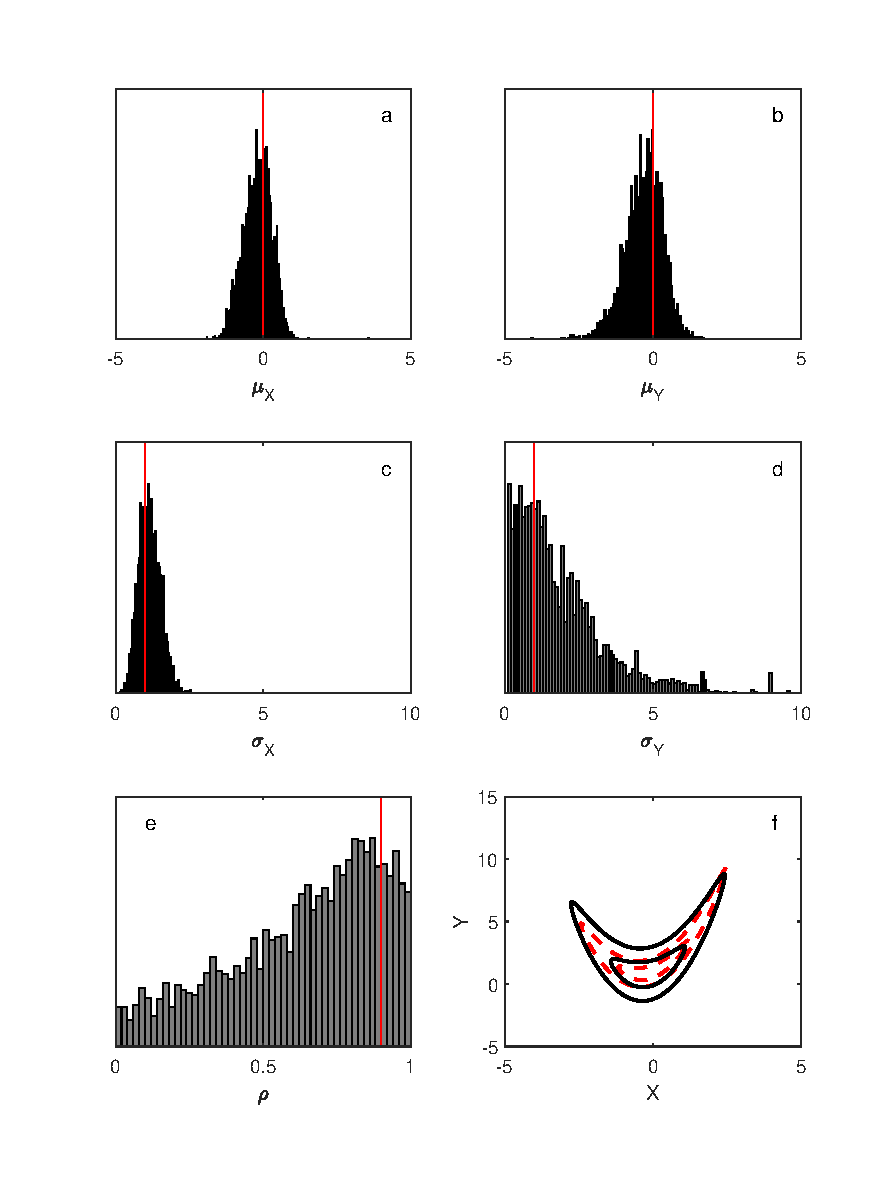
\includegraphics[scale=1.1]{bananaABC-MH.pdf}
	\caption{The marginal posterior distributions for banana parameter inference, as well as the median posterior model (f), in black, compared to the causative model, red dashed lines. Red lines mark the true parameter values on the marginal posterior plots. I justify the legitimacy of extracting the median marginal model as there are limited correlations between the unknown parameters, figure \ref{correlation-plot}.}
	\label{MH-banana}
\end{figure}

% Insert correlation plot of 5 pars to justify taking the MLE
\begin{figure}[H]
	\centering
	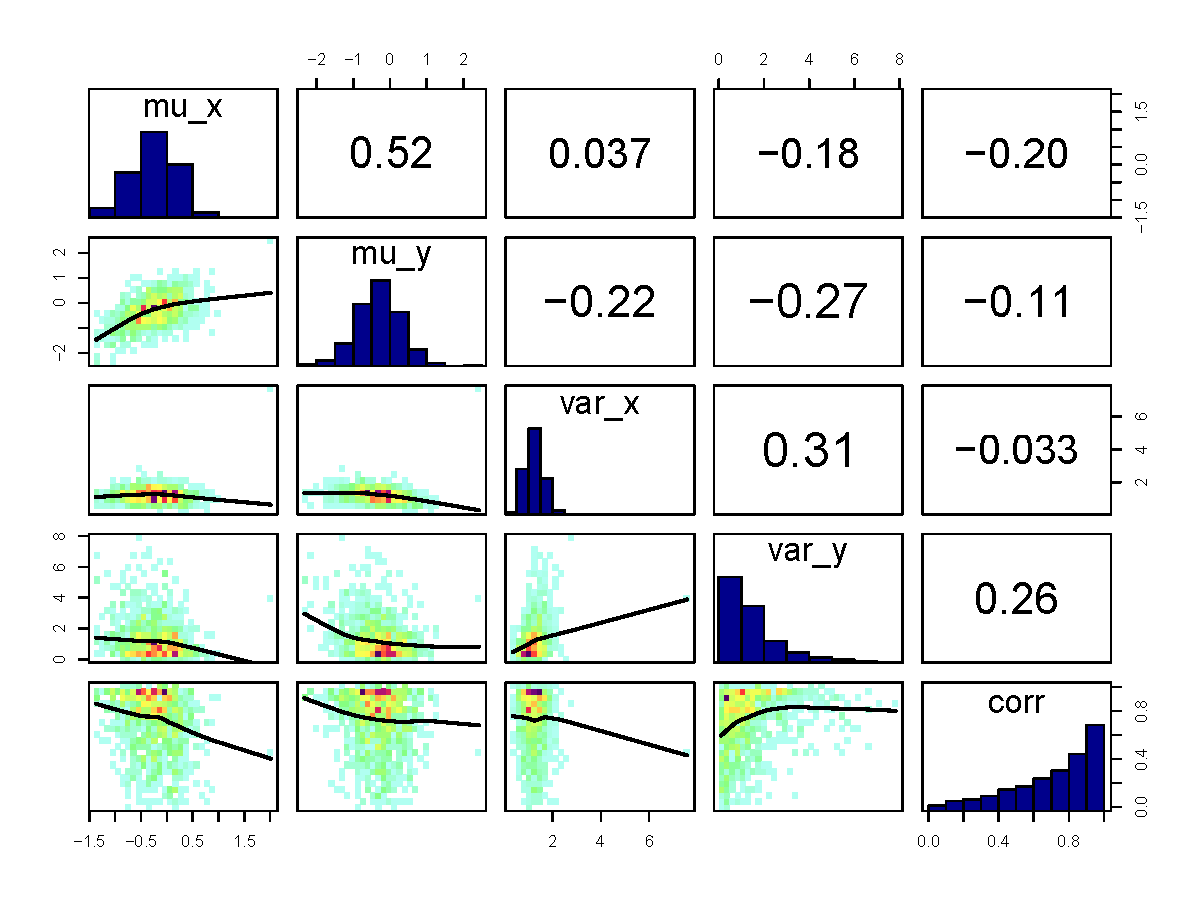
\includegraphics[scale=0.6]{correlationplot.pdf}
	\caption{The panels visualize correlations between parameters in the posterior sampled by the Markov chain in figure \ref{MH-banana}. The diagonal shows the marginal distributions which are also plotted in figure \ref{MH-banana}(a)(b)(c)(d)(e). The lower triangle shows the correlation density between the parameter on the diagonal (red marks higher density) and a polynomial fit to the correlation (black line). The upper triangle shows Spearman's rank correlation coefficients for the correlations in the lower triangle. There is limited correlation between the parameters, as indicated by the low Spearman's rank values and broadly distributed correlation density. This is used as justification for plotting statistics of the posterior marginal distributions as representative of the joint posterior distribution.}
	%\caption{Correlation plot for the Markov chain in figure \ref{MH-banana}. There is limited correlation between the parameters. This is used as justification for plotting statistics of the marginal posterior as representative of the joint posterior.}
	\label{correlation-plot}
\end{figure}

The performance of the MCMC algorithm as described by algorithm \ref{ABC-MCMC} depends on the users ability to choose a suitable proposal distribution $q(\cdot,\cdot)$. If the proposal distribution is limited to a multivariate Gaussian distribution, then a suitable covariance matrix must be chosen. If the variance for each parameter is too large then the probability of accepting a candidate move will be low, as each step will be erratic and far from the current location. Consider that as the variance for $q(\cdot,\cdot) \rightarrow \infty$ we effectively have a Monte Carlo scheme. However, if the variance is too small then the acceptance rate will be very high but the algorithm will fail to explore the full parameter space. We desire both a reasonable acceptance rate and a good exploration of the parameter space. The variance is selected to explore the posterior distribution efficiently. It is very difficult to set the correlation between parameters, the off-diagonal terms in the covariance matrix, a priori. It is also time consuming and difficult to tune the correlation values. Generally, it is simplest to leave the correlations set to zero. \par

However, such a system is not ideal. Selecting an optimal proposal distribution is non-trivial problem. Here we can turn to theoretical developments to guide a better proposal distribution. \citet{Gelman1996} show that when the target distribution is Gaussian, an efficient sampler can be constructed by scaling the proposal covariance to $2.4^2/d$, where $d$ is the number of unknown parameters. In the previous sections it has been best to ignore the correlations between parameters. However, these correlations can be important to consider, if there are strong parameter correlations in the posterior then sampling acceptance rate will be lowered and convergence undermined. Ideally the algorithm should be able to learn about the posterior on the fly, and if there are correlations between parameters, adjust accordingly. With this in mind \citet{haario2001} developed Adaptive Metropolis (AM). AM tunes the proposal distribution to the posterior distribution by using the history of the chain generated up to the current time. After some designated time, $t$, the covariance matrix of the proposal distribution, $\bm{\Sigma_q}$, is set to the covariance of the Markov chain. 
\begin{equation}
\bm{\Sigma_q} = \text{cov}(\bm{\theta}_1,\dots,\bm{\theta}_t)s_{AM} + I\upsilon
\end{equation}
Where $s_{AM}$ is the scaling factor, generally $2.4^2/d$, and $\upsilon$ is a small positive which prevents the covariance from becoming singular. AM sampler efficiency is compared to MH in table \ref{sampling-method-comparison}.\par

Figure \ref{AM-demonstration} plots the effect AM has on a sub-optimal choice for a proposal distribution.\par

In this example a 4-stage adaptive scheme is used over the length of the chain. Figure \ref{4-stage-am} plots this scheme. With this in mind, Figure \ref{AM-demonstration} plots the proposal distribution before the first adaption, red, and after the 4th adaption, blue. \\
\linebreak
\linebreak
\linebreak

\begin{figure}[h]
%\vspace{2cm}
\begin{minipage}{1.0\linewidth}
\centering
    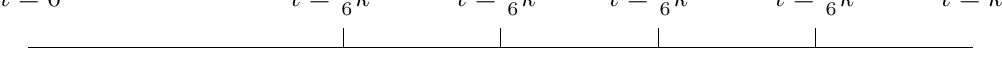
\begin{tikzpicture}
	\draw (0,0) -- (12,0);
	\draw (4,0) -- (4,0.25);
	\draw (6,0) -- (6,0.25);
	\draw (8,0) -- (8,0.25);
	\draw (10,0) -- (10,0.25);

	\put(-10,15){$t = 0$}
	\put(95,15){$t = \frac{2}{6}k$}
	\put(155,15){$t = \frac{3}{6}k$}
	\put(210,15){$t = \frac{4}{6}k$}
	\put(270,15){$t = \frac{5}{6}k$}
	\put(330,15){$t=k$}

	\put(108,50){$1^{st}$}
	\put(95,40){$adaption$}
	\put(163,40){$2^{nd}$}
	\put(220,40){$3^{rd}$}
	\put(277,40){$4^{th}$}
    \end{tikzpicture}
\end{minipage}

\caption{4-stage adaptive scheme for a Markov chain of length $k$}
\label{4-stage-am}
\end{figure}

\begin{figure}[H]
	\centering
	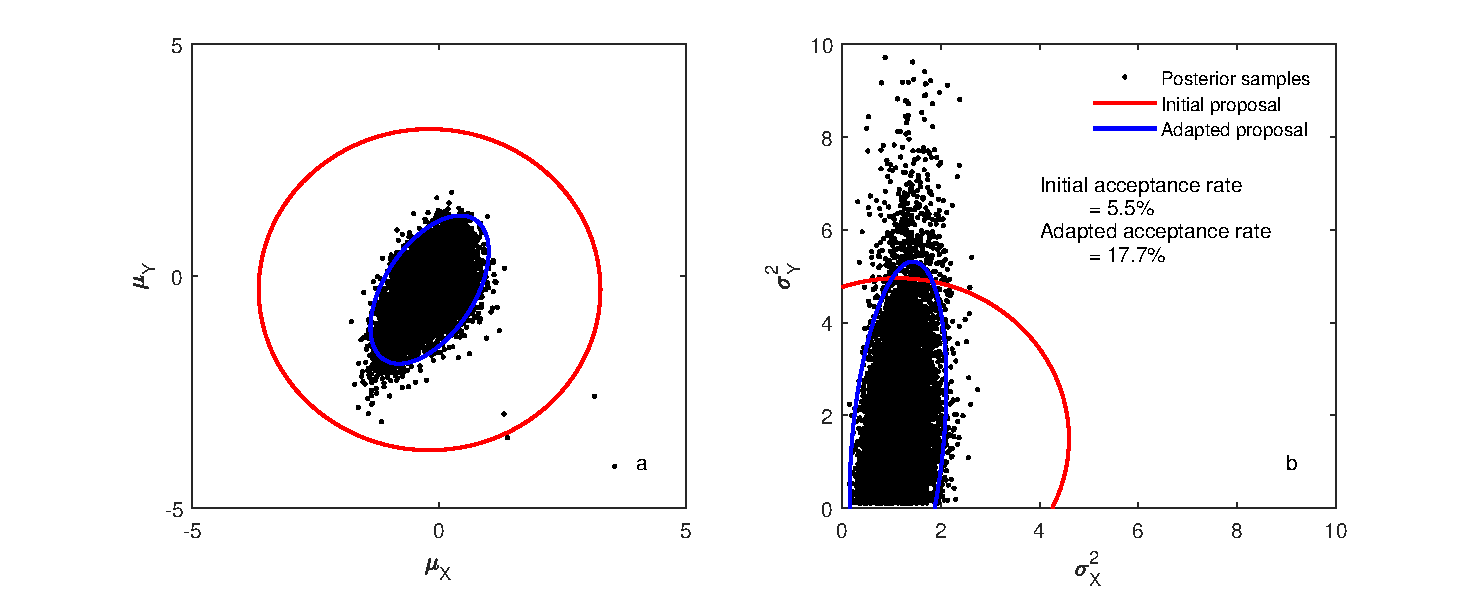
\includegraphics[scale=0.7]{amdemonstration.pdf}
	\caption{Adapted proposal distribution compared to a suboptimal initial proposal. This suboptimal choice was the proposal distribution of the MCMC algorithm in figure \ref{MH-banana}.}
	\label{AM-demonstration}
\end{figure}

Delayed Rejection (DR) can also be implemented to improve sampling efficiency \citep{Mira2001}. Under DR, when a proposed move is rejected, instead of advancing a time step and retaining the same position, another proposed candidate move is considered. The acceptance probability of the second proposal differs from the MH acceptance probability in order to retain time reversibility of the Markov chain, ensuring that the chain converges to the desired stationary distribution. When a Markov chain remains in the same position over time, the estimates obtained by averaging along the chain become less accurate. Increases to the autocorrelation of the chain increase the variance of estimates based on the chain \citep{Mira2001}. In this way DR gives more reliable estimates than a standard MH algorithm. A two-stage DR algorithm, as is applied in this text, operates as follows. \par

At the first stage the acceptance probability is the Metropolis-Hastings acceptance probability:
\begin{equation}
	\alpha_1(\theta,\theta^*) = \text{min}\bigg\{1,\frac{\pi(\theta^*)q_1(\theta^*,\theta)}{\pi(\theta)q_1(\theta,\theta^*)} \bigg\}
\end{equation}
where $\pi$ is the target distribution of the algorithm and $q_1$ is the proposal distribution. If the proposed move to $\theta^*$ is rejected then a second candidate move, $\theta^{**}$, can be considered from the second proposal distribution $q_2$. The acceptance probability for $\theta^{**}$ is:
\begin{equation}
	\alpha_2(\theta,\theta^*,\theta^{**}) = \text{min}\bigg\{1,\frac{\pi(\theta^{**})q_1(\theta^{**},\theta)q_2(\theta^{**},\theta^*,\theta)[1-\alpha_1(\theta^{**},\theta^*)]}{\pi(\theta)q_1(\theta,\theta^*)q_2(\theta,\theta^*,\theta^{**})[1-\alpha_1(\theta,\theta^*)]} \bigg\}
\end{equation}
Here I limit implementation to a two-stage DR scheme and use a $q_2$ with a smaller covariance matrix. $q_1$ is downscaled to give $q_2$ by the relation, $q_2 = q_1/s_{DR}$. DR is compared to MH and AM in table \ref{sampling-method-comparison}.\par

Both Adaptive Metropolis and Delayed Rejection can be implemented together to give a Delayed Rejection Adaptive Metropolis scheme \citep{Haario2006}. There are many implementation possibilities given the mixing of AM and DR. A straight forward implementation is favoured, as in \citet{Laine2008}, which retains the principal advantages of each method to give an efficient adaptive algorithm.    The first stage proposal is adapted to the chain generated so far, and one scaled down second stage proposal is considered. The second stage proposal inherits the adapted covariance matrix of the first stage proposal, only the variances are reduced. DRAM is compared to MH, AM and DR in table \ref{sampling-method-comparison}.\par

When running a 'one-size fits all' generic MCMC algorithm, the standard procedure is to propose a candidate move which updates each and every parameter value. If we are at the position $\bm{\theta_{t-1}}$ in the parameter space, then the proposal distribution suggests a candidate move:
\begin{equation}
	\bm{\theta_{t}} = \mathcal{N}(\bm{\theta_{t-1}},\bm{\Sigma_q})
\end{equation}
However, this is not the only option. Another choice is to update a single parameter per time step. The choice to update one, or all parameters are end members on a spectrum of updating some sub-set of all parameters. This technique is referred to as parameter blocking \citep{Roberts1997,Sargent2000}. Much like the variance of $\bm{\Sigma_q}$, there is a trade-off between acceptance rate and speed of parameter space exploration encoded into this decision. Table \ref{sampling-method-comparison} compares the acceptance rate of a MH algorithm where all parameters are updated at once, and an MH algorithm where a single parameter is updated per time step. A significant increase in acceptance rate is made through this change. However, while acceptance rate is increased, the speed of parameter space exploration is slowed. Effective parameter blocking requires problem specific implementation and tuning. 

\begin{table}[H]
	\centering
	\begin{tabular}{|c|c|}
	\hline
	Sampling method & Acceptance rate (\%) \\
	\hline
	Metropolis-Hastings (MH) & 5.43\% \\
	\hline
	Adaptive Metropolis (AM) & 13.35\% \\
	\hline
	Delayed Rejection (DR) & 23.04\% \\
	\hline
	Delayed Rejection Adaptive Metropolis (DRAM) & 36.42\% \\
	\hline
	Single parameter update & 43.7\% \\
	\hline
	\end{tabular}
	\caption{Comparison of sampler efficiency for the banana parameter estimation problem. The sampled posterior is the same for each method. The AM and DRAM acceptance rate is taken over the full length of the chain. Each chain is of length $t = $ 1,000,000.}
	\label{sampling-method-comparison}
\end{table}

While ABC targets the underlying parameters to the banana distribution, there is also access to the probability density of the causative model. With access to the causative models probability in $X-Y$ space it is possible to run a Markov chain to discover the distribution. Figure \ref{Analytical-banana}(a) plots a Markov chain with the stationary distribution of the causative model, black dots, as well as the 50\% and 95\% confidence intervals of the causative model. The Markov chain can be used for kernel density estimation of the causative model, figure \ref{Analytical-banana}(b). With this in mind it is possible to compare the estimation of the causative model with ABC and under access to the analytical probability density. Figure \ref{the-comparison} compares the estimation of the causative model based on a standard MH algorithm (a), AM (b), DR (c), DRAM (d), and ABC-MH (e), ABC-AM (f), ABC-DR (g), ABC-DRAM (h). 

\begin{figure}[H]
\centering
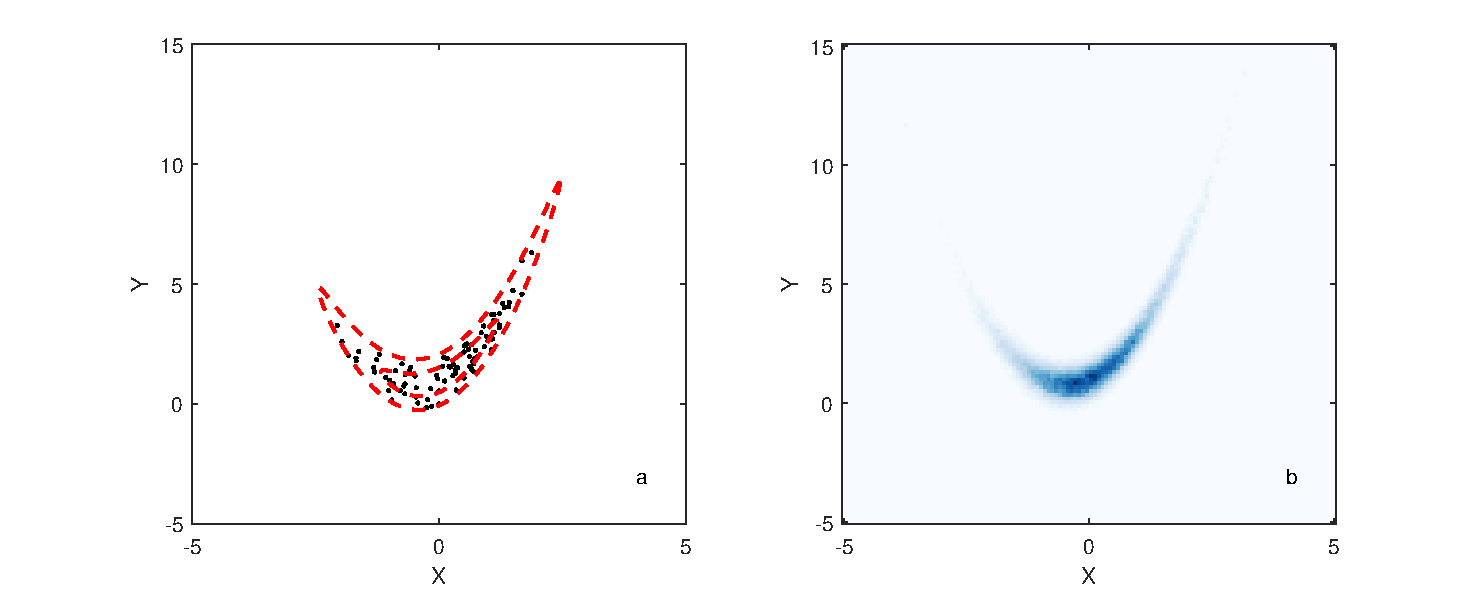
\includegraphics[scale=0.7]{analyticaltestplot.pdf}
\caption{A Metropolis-Hastings algorithm sampling the causative model. (a) The MCMC samples, black dots, to the causative model. Red dashed lines mark the 50\% and 95\% confidence intervals of the causative model. (b) kernel density estimation based on the MCMC samples. Kernel density estimation in 2d is based on the diffusion algorithm of \citet{Botev2010}.}
\label{Analytical-banana}
\end{figure}

Throughout this example a strong trend has emerged. The acceptance rate of a Markov chain based algorithm targeting the ABC posterior is strongly tied to the tolerance. This shows the effect of tolerance in a rejection scheme is persistent, and generalizes to more advanced samplers. Increasing the tolerance increases the acceptance rate, while decreasing the tolerance decreases the acceptance rate. With this in mind, the improvements to the acceptance rate of ABC-MCMC offered by AM, DR, single parameter updates and blocking are very important for sampling the most accurate posterior possible. With each improvement to acceptance rate the tolerance can be lowered while still remaining in the realm of reasonable sampler efficiency, around 10-30\% acceptance rate. So far all comparisons have been done using a tolerance $\epsilon =\begin{bmatrix}
0.625\ 0.625\ 0.625\ 0.625\ 0.625\ 0.125\ 0.625\ 0.625
\end{bmatrix}^T$ 
for the statistic set $\begin{bmatrix}
\bar{\mu_X}\ \bar{\sigma_X}\ \bar{\gamma_Y}\ \bar{\mu_Y}\ \bar{\sigma_Y}\ a\ b\ c
\end{bmatrix}^T$. This tolerance is used to keep ABC-MH, the worst performing sampler, computationally feasible. However, using ABC-DRAM with single parameter updates it is possible to lower the tolerance to 
$\epsilon = \begin{bmatrix}
0.01\ 0.01\ 0.01\ 0.01\ 0.002\ 0.01\ 0.01\ 0.01
\end{bmatrix}^T$
while still remaining within the limits of computational feasibility. Figure \ref{best-banana} plots this scenario. With ABC-DRAM and single parameter updates the acceptance rate is ~7\% under this tolerance. While ABC-MCMC sampling, with all parameter updates, becomes computationally infeasible with an acceptance rate <0.3\%.

\begin{figure}[H]
\centering
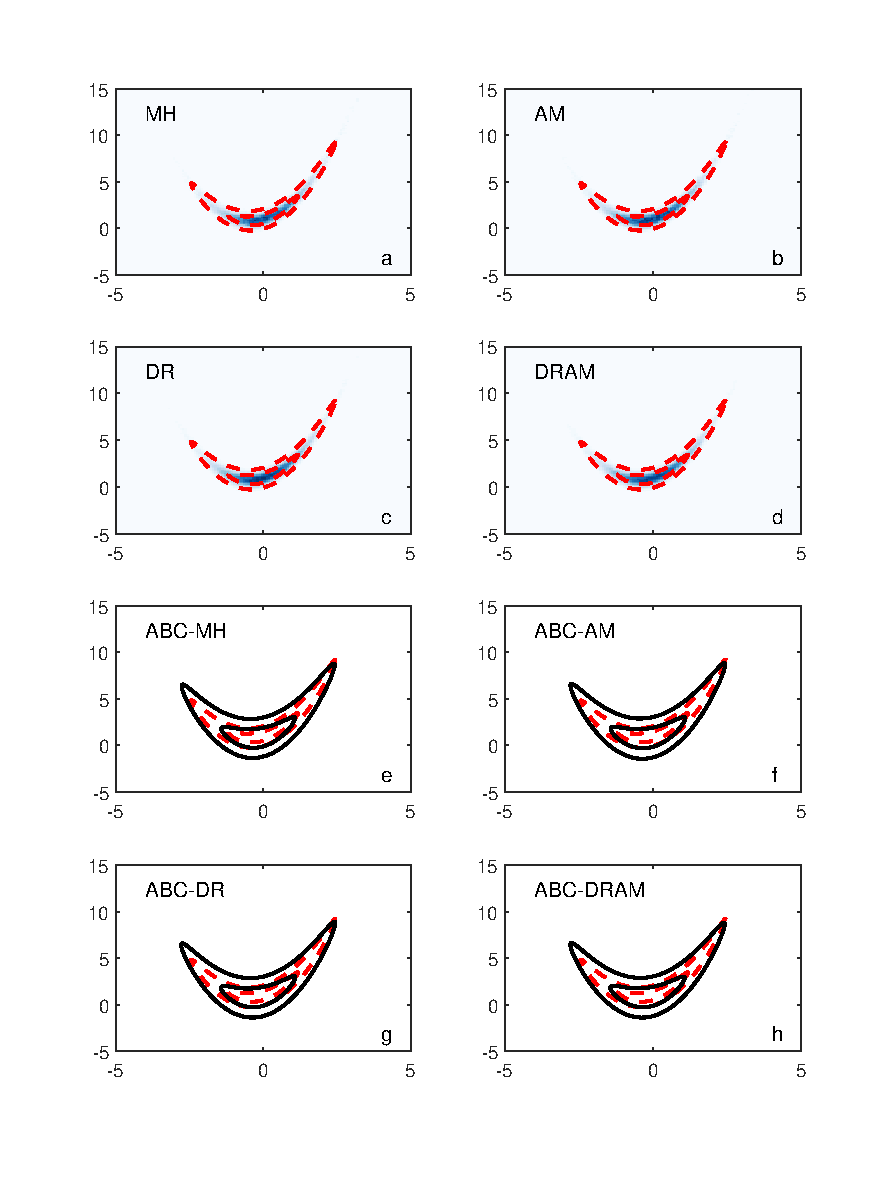
\includegraphics[scale=1.15]{abcanacomparison.pdf}
\caption{Comparison of estimation of the causative banana model based on access to the analytical formula (a,b,c,d) and no access to the analytical formula (e,f,g,h), simply simulation from the model.}
\label{the-comparison}
\end{figure}

\begin{figure}[H]
\centering
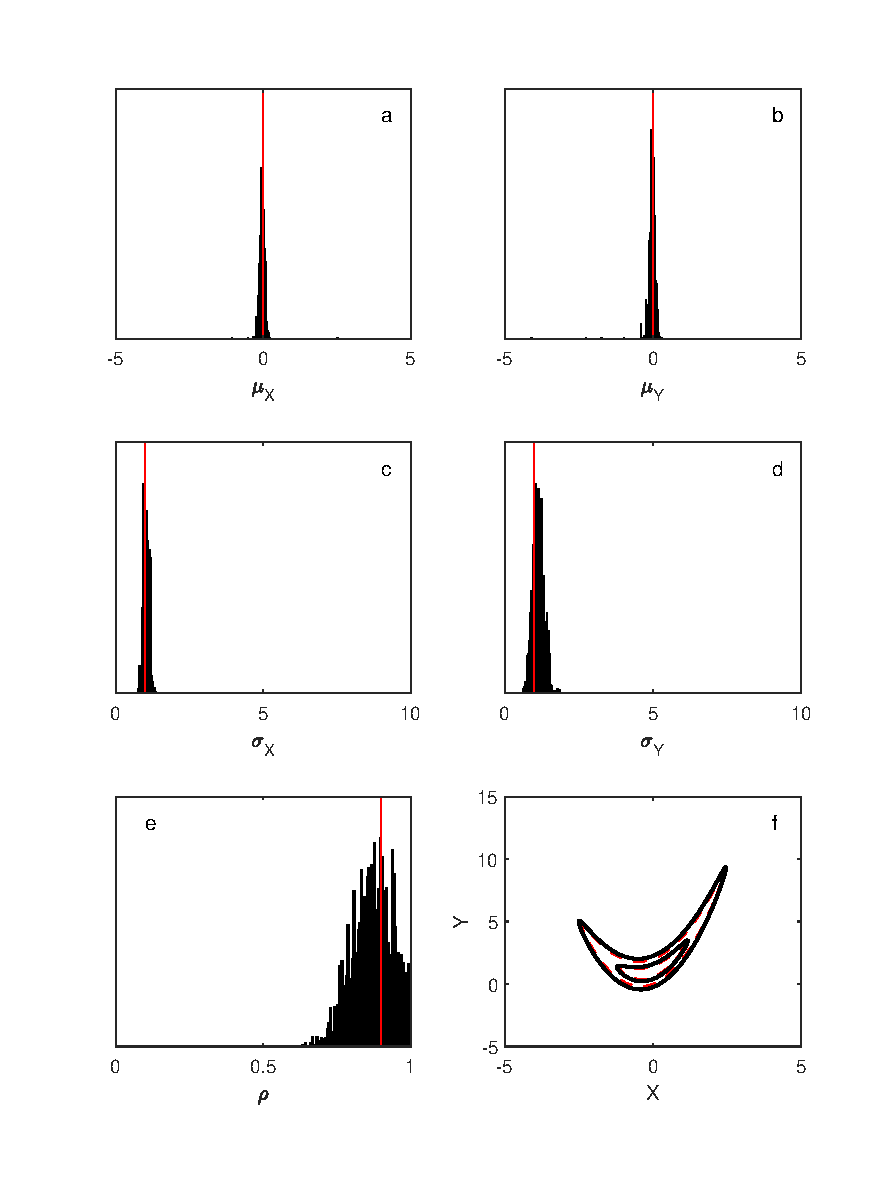
\includegraphics[scale=1.1]{bananaABC-DRAM.pdf}
\caption{Banana parameter estimation based on ABC-DRAM with single parameter updates. The tolerance is lowered, see text for tolerance values. By lowering the tolerance inference is more accurate. Compared to \ref{MH-banana} the marginal posteriors are more tightly clustered around the true solution and the median marginal model, black lines of (f) fit the causative model, red dashed lines, far better.}
\label{best-banana}
\end{figure}